% Created 2019-04-17 Wed 18:20
\documentclass[a4paper]{article}
\usepackage[utf8]{inputenc}
\usepackage[T1]{fontenc}
\usepackage{fixltx2e}
\usepackage{graphicx}
\usepackage{longtable}
\usepackage{float}
\usepackage{wrapfig}
\usepackage{rotating}
\usepackage[normalem]{ulem}
\usepackage{amsmath}
\usepackage{textcomp}
\usepackage{marvosym}
\usepackage{wasysym}
\usepackage{amssymb}
\usepackage{hyperref}
\tolerance=1000
\date{}
\title{A simple fat tree network showcase}
\hypersetup{
  pdfkeywords={},
  pdfsubject={},
  pdfcreator={Emacs 25.2.2 (Org mode 8.2.10)}}
\begin{document}

\maketitle
\section*{Course}
\label{sec-1}
Fog and Cloud Computing 2018/2019
\section*{Students}
\label{sec-2}
\begin{itemize}
\item Brugnera, Lorenzo <lorenzo.brugnera@studenti.unitn.it>, S197054
\item Zaupa, Eros <eros.zaupa@studenti.unitn.it>, S208272
\end{itemize}
\section*{Proposal}
\label{sec-3}
Our project goal is to reproduce a model of a fat tree network using
the OpenStack service. Fat tree networks are usually deployed in
environments with \emph{high} computational power and \emph{heavy} bandwidth
consumption, such us \emph{data centers} and \emph{cluster supercomputers}. The
resources made available by the OpenStack service can't compare to the
requirements of real use cases, but a \emph{simpler} and \emph{lighter}
implementation of this topology is still feasible. The model will
cover the main property of the topology: top branches are "fatter"
(thicker) than lower branches. This means that for each \emph{edge} switch,
the number of links that go to its siblings is equal to the number of
links that go to its parents.
\subsection*{Configuration}
\label{sec-3-1}
We will use \emph{\href{https://www.ansible.com/}{Ansible}} as an automation tool for two main reasons
\begin{enumerate}
\item The available OpenStack service comes with \emph{no guarantees}, so
preventing any data loss is up to us.
\item We want to define the project configuration in a \emph{structured} way.
\end{enumerate}
\subsection*{Network}
\label{sec-3-2}
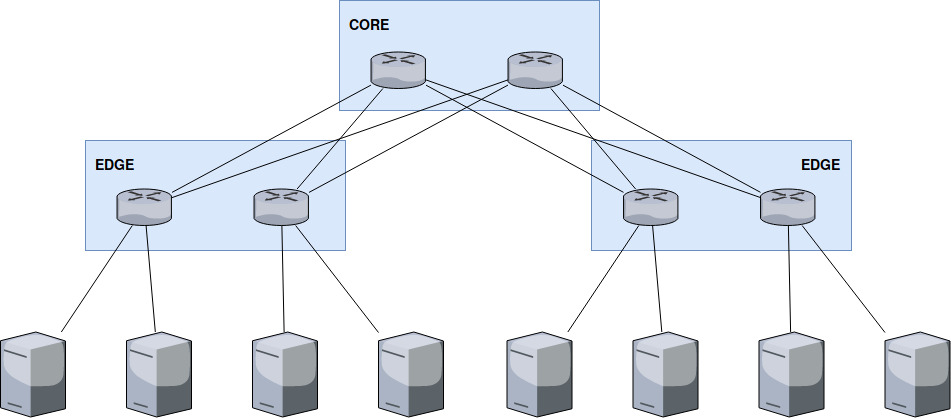
\includegraphics[width=.9\linewidth]{./network.jpg}
\begin{itemize}
\item $L=2$ level fat tree.
\item $K=4$ ports per switch.
\item $(2L-1)(K/2)^{L-1}=3(K/2)=6$ switches.
\begin{itemize}
\item $(K/2)^{L-1}=K/2=2$ \emph{core} switches.
\item $2(K/2)^{L-1}=K=2$ \emph{edge} switches.
\end{itemize}
\item $N=2*(P/2)^L=8$ hosts.
\end{itemize}
\subsection*{Requirements}
\label{sec-3-3}
\begin{description}
\item[{Instances}] To keep the resources consumption at minimum, our goal
is to use a \emph{m1.tiny} flavor for each instance running
an OS with low requirements (e.g. CirrOS) using 8 of
the 10 instances slots available. This should be enough
to execute simple connection tests (e.g. ping, ssh).
\item[{Routers}] We will use 6 of the 10 routers slots available.
\end{description}
\subsection*{References}
\label{sec-3-4}
\begin{itemize}
\item \url{https://clusterdesign.org/fat-trees/}
\item \url{https://www.cs.cornell.edu/courses/cs5413/2014fa/lectures/08-fattree.pdf}
\item \url{https://packetpushers.net/demystifying-dcn-topologies-clos-fat-trees-part2/}
\item \url{https://www.ansible.com/}
\end{itemize}
% Emacs 25.2.2 (Org mode 8.2.10)
\end{document}
